\documentclass[runningheads,a4paper]{llncs}

\usepackage{booktabs}
\usepackage{multirow}
\usepackage{lscape}
\usepackage{geometry}
\usepackage{amsmath}
\usepackage{amssymb}
\setcounter{secnumdepth}{4}
\setcounter{tocdepth}{4}
\usepackage{graphicx}
\usepackage{url}

% Configuración de UTF-8 para poder escribir en Español
\usepackage[utf8]{inputenc}
\usepackage[spanish]{babel}

% Configuración de Citas
\usepackage[numbers]{natbib}
\bibliographystyle{plainnat}
\selectlanguage{spanish}

% Configuración de Listing (para mostrar código en LaTeX).
\usepackage{listings}
\usepackage{color}
 
\definecolor{codegreen}{rgb}{0,0.6,0}
\definecolor{codegray}{rgb}{0.5,0.5,0.5}
\definecolor{codepurple}{rgb}{0.58,0,0.82}
\definecolor{backcolour}{rgb}{0.95,0.95,0.92}
 
\lstdefinestyle{default_style}{
    backgroundcolor=\color{backcolour},   
    commentstyle=\color{codegreen},
    keywordstyle=\color{magenta},
    numberstyle=\tiny\color{codegray},
    stringstyle=\color{codepurple},
    basicstyle=\footnotesize,
    breakatwhitespace=false,         
    breaklines=true,                 
    captionpos=b,                    
    keepspaces=true,                 
    numbers=left,                    
    numbersep=5pt,                  
    showspaces=false,                
    showstringspaces=false,
    showtabs=false,                  
    tabsize=2
}
 
\lstset{style=default_style}

\begin{document}

\mainmatter

\title{Sondeo del estado del arte en TCP Incast}
\author{Julián Bayardo}
\institute{Universidad de Buenos Aires\\
\url{julian@bayardo.info}}

\maketitle

\tableofcontents

\newpage

\section{Introducción}

Una de las claves del desarrollo de Internet en los últimos años ha sido lograr escalar la infraestructura para soportar los millones de usuarios nuevos y sus dispositivos. Desde el punto de vista de los proveedores de servicios, el cómputo en la nube ha sido la clave para lograrlo, y los \textit{data centers} el medio facilitador.

Aunque no hay una definición estandarizada de qué es un \textit{data center}, el consenso es que el término hace referencia a una red de servidores con ciertas garantías de tolerancia a fallas (tanto en \textit{storage} como en la red), escalabilidad horizontal, y uniformidad en sus capacidades de procesamiento y transferencia de datos.

Usos populares en \textit{data centers} destinados a infraestructura en la nube son, por ejemplo, el de cómputo distribuido que sigue el paradigma MapReduce\cite{Dean_MapReduce_2004}, o los sistemas de \textit{storage} distribuidos como HDFS\cite{Shvachko_HDFS_2010}. En este tipo de aplicaciones en línea y de uso intensivo de datos, se hace uso de alto paralelismo a través de una metodología de trabajo \textit{divide and conquer}.

Las peculiaridades de infraestructura junto con este tipo de aplicación en particular generan un ecosistema único. Desde la infraestructura, vemos \cite{Benson_Network_2010}:

\begin{itemize}
\item Topología en forma de árbol con múltiples raíces, y regular en el número de conexiones con los sub-árboles.

\item Los switches y routers que se utilizan son baratos y fáciles de conseguir, implicando en particular que tienen buffers pequeños.
\end{itemize}

Y, desde el punto de vista de la comunicación entre servidores:

\begin{itemize}
    \item Las conexiones suelen ser de muchos hacia uno, de banda ancha, y baja latencia. Esto sucede durante la etapa de agregación de los algoritmos \textit{divide and conquer}.
    
    \item En 80\% de los casos, el tráfico se queda dentro del mismo rack, es decir, es altamente localizado a un subárbol, y además no sale de la red interna.
\end{itemize}

En concreto, los \textit{data centers} tienen condiciones operativas ampliamente diferentes a las que tiene el resto de la Internet y, sin embargo, a priori utilizan el mismo \textit{stack} de protocolos; dejando claro una oportunidad para una mejora de \textit{performance} significativa. Es por esto que los últimos años han visto una gran cantidad de investigación en torno a cómo adaptar el \textit{stack} para funcionar mejor en \textit{data centers}.

Siguiendo estos lineamientos, este trabajo tiene como objetivo poner el foco en la utilización de TCP en los \textit{data centers}, y en particular sobre el problema de TCP Incast que se genera utilizando MapReduce. Haremos un relevamiento de la literatura en torno a las posibles formas de evitarlo, y la experiencia práctica que se tiene con las mismas.

El resto de este trabajo se estructura de la siguiente forma: en la Secc. \ref{problems} introduciremos algunos de los problemas observados en las \textit{data center networks} (DCNs) y sus causas. Luego, pondremos el foco exclusivamente en TCP Incast para realizar un análisis de las distintas formas de mitigar el problema en la Secc. \ref{solutions}. Finalmente, concluimos en la Secc. \ref{conclusion}. 

\section{Problemas de TCP en Data Center Networks} \label{problems}

\subsection{Introducción a Map Reduce}

\begin{figure}[b!]
    \centering
    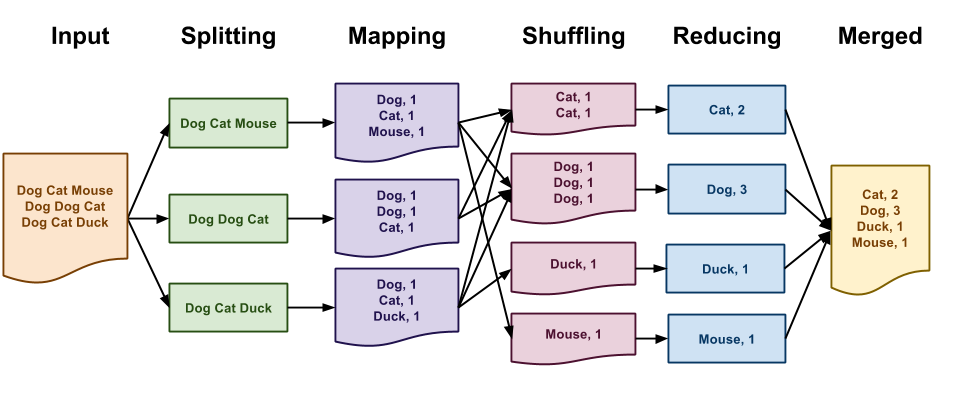
\includegraphics[width=1\textwidth]{figures/MapReduce_Example.png}
    \caption{MapReduce aplicado para resolver el problema de conteo de palabras}
    \label{fig:mapreduce_example}
\end{figure}

La arquitectura de procesamiento paralelo MapReduce se divide en dos etapas, Map y Reduce. Durante la primer etapa, la entrada a procesar se transforma en un conjunto de pares clave-valor. En la segunda etapa, el conjunto de pares generado por la etapa anterior se ordena por clave, y se envía, agrupado por clave, a cada nodo para aplicar una función de agregación entre los valores con la misma clave.

En el ejemplo de la figura \ref{fig:mapreduce_example}, buscamos contar la cantidad de ocurrencias de una palabra en un corpus de textos. Para resolver este problema utilizando una arquitectura MapReduce, precisamos de una función de map, y otra de reduce, escritas en Haskell:

\begin{lstlisting}[language=Haskell]
mapper :: String -> [(String, Int)]
mapper = fmap (\word -> (word, 1)) . words

reducer :: String -> [Int] -> Int
reducer key = sum
\end{lstlisting}

La arquitectura se encargará automáticamente de distribuir la ejecución de \verb|mapper| sobre todos los nodos del cluster, lo mismo con \verb|reducer|, y finalmente de o bien guardar, o bien transmitir los resultados finales de la ejecución a un último nodo. Desde el punto de vista de la red, tenemos tres puntos claves de comunicación:

\begin{enumerate}
    \item Cuando en un comienzo se distribuye el conjunto de datos entre múltiples nodos, lo que requiere que los mismos puedan leerlo y aplicar la función \verb|mapper|.
    
    \item Luego de la etapa de Map, cuando debemos agrupar los pares por clave y enviarlas a sus respectivos nodos
    
    \item Y finalmente, cuando termina la etapa de Reduce, cada nodo debe escribir sus resultados a un sistema de \textit{storage}.
\end{enumerate}

Durante el resto de este trabajo nos focalizaremos, por motivos que van a ser aparentes luego, en mecanicas como las del punto número 2. Observemos que el patrón generado por el mismo es claramente de muchos a uno (específicamente, de algún subconjunto de mappers a el nodo de reduce para una clave dada).

Más aun, este tipo de utilización de la red es común también en los sistemas de \textit{storage} distribuidos. De hecho, es en este mismo tipo de aplicaciones que fueron descubiertos y nombrados los problemas que nos conciernen \cite{Nagle_Panasas_2004}.

\subsection{TCP Incast}

\begin{figure}[b!]
    \centering
    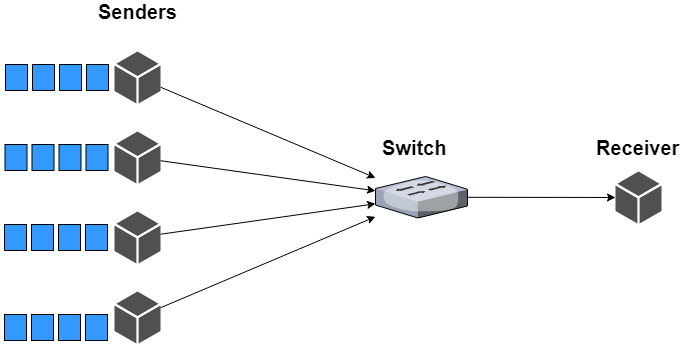
\includegraphics[width=1\textwidth]{figures/TCP_Incast_Pattern.png}
    \caption{Patrón abstracto de TCP Incast. Los senders envían paquetes de un tamaño fijo hacia un switch que funciona como cuello de botella para el \textit{receiver}}
    \label{fig:tcp_incast_pattern}
\end{figure}

TCP Incast es un comportamiento patológico de TCP, producido en patrones de comunicación de muchos a uno, donde se observa una caída rápida del \textit{goodput} a nivel de aplicación. Hay una gran cantidad de trabajos de investigación que han investigado el motivo por el cual esto sucede. El patrón de comunicación es el siguiente\cite{Phanishayee_Throughput_2008}\cite{Qin_TCP_2016}:

\begin{enumerate}
    \item Un cliente le pide a un conjunto de servidores que estos le envíen alguna pieza de información.
    
    \item Los servidores responden todos al mismo tiempo con los datos solicitados, en el estilo de la figura \ref{fig:tcp_incast_pattern}.
\end{enumerate}

Durante el paso uno, el cliente requiere una cantidad de información de tamaño \textit{Block Size} (B), que está en el orden de 1MB. Para esto, a cada servidor le solicita un fragmento de tamaño \textit{Server Request Unit} (SRU), en el orden de 32KB. El cliente debe recibir todos los SRU para considerar que se completó la solicitud del bloque. Además, el cliente no emitirá ninguna otra solicitud hasta haber completado la actual.

Recordemos que el 80\% del tráfico en los \textit{data centers} se mantiene dentro del mismo \textit{rack}, es decir, gran parte del tráfico pasa por el mismo \textit{switch}. Durante el paso dos; este \textit{switch}, ante el volumen de paquetes que recibe en salida hacia el puerto donde se localiza el cliente, termina quedándose sin lugar en el \textit{buffer}, y por ende comienza a descartar paquetes.

TCP detecta esto, desde el lado de los servidores, cuando observa que no recibe ACKs para los paquetes que envió (o, alternativamente, que recibe ACKs duplicados). Lo primero genera que la ventana de congestión se reduzca, y además genera una retransmisión de los paquetes por haber recibido un \textit{timeout}, mientras que lo segundo solamente una retransmisión. 

Estos \textit{timeouts} imponen una espera de cientos de milisegundos, en redes cuyo RTT está en decenas a cientos de microsegundos, de esta manera desatando la caída del \textit{goodput}: el tráfico de la red queda dominado por los tiempos de espera de TCP ante la necesidad de retransmitir paquetes.

Concretamente, TCP Incast es un problema que surge de una interacción sutil entre el tamaño de \textit{buffer} de los Ethernet \textit{switches} (capa de enlace), los mecanismos de recuperación de pérdidas de TCP (capa de transporte), y patrones de comunicación caracteristicos de las aplicaciones típicas de un data center (capa de aplicación).

\subsection{TCP Outcast}

TCP Outcast es otro comportamiento patológico, pero en términos de \textit{fairness} a nivel de capa de enlace \cite{Prakash_Outcast_2012}. En este caso, un conjunto de puertos en un \textit{switch} son "dejados de lado" (\textit{outcast}), es decir, obtienen un porcentaje menor del ancho de banda disponible en comparación con otros puertos. Esto se reifica en una gran cantidad de \textit{timeouts} percibidos por TCP, generando entonces un colapso de la ventana de congestión.

Analizando un modelo teórico de TCP Reno, puede verse que el \textit{throughput} es inversamente proporcional al RTT entre los hosts \cite{Padhye_TCP_Throughput_1998}. Cuando se produce TCP Outcast, exactamente lo contrario sucede: es un patrón de comunicación de muchos a uno, donde \textit{senders} que tienen menor RTT al \textit{receiver} observan \textit{throughput} hasta un orden de magnitud menor que los que están a mayor RTT; más aun, esto empeora cuando la cantidad de conexiones del host a menor RTT aumentan.

Esencialmente, para que se produzca TCP Outcast deben suceder dos condiciones clave:

\begin{enumerate}
    \item Los \textit{switches} deben utilizar un esquema de \textit{tail drop} para manejar las colas de paquetes. Es decir, deben descartar los paquetes intentando entrar a la cola cuando esta se llena.
    
    \item Dos conjuntos de conexiones, uno grande y uno chico, deben estar llegando en dos puertos de entrada distintos, y estar compitiendo por el mismo puerto de salida, que resulta ser el cuello de botella.
\end{enumerate}

La primer condición se cumple ampliamente en los data centers, dado que utilizan \textit{switches} que no son específicos para el propósito. Por otro lado, la segunda condición suele cumplirse como un efecto secundario de las arquitecturas distribuidas.

En su conjunto, las dos condiciones generan un fenómeno, denominado Port Blackout, por el cual la cola de salida del \textit{switch} para el puerto del \textit{receiver} se queda casi llena, y los paquetes de las conexiones con mayor RTT llenan la cola hasta el tope. Luego, se intenta encolar uno o más paquetes de la conexión con menor RTT, y estos son descartados automáticamente porque no entran en la cola. En la figura \ref{fig:port_blackout_example} puede verse un ejemplo.

\begin{figure}[t!]
    \centering
    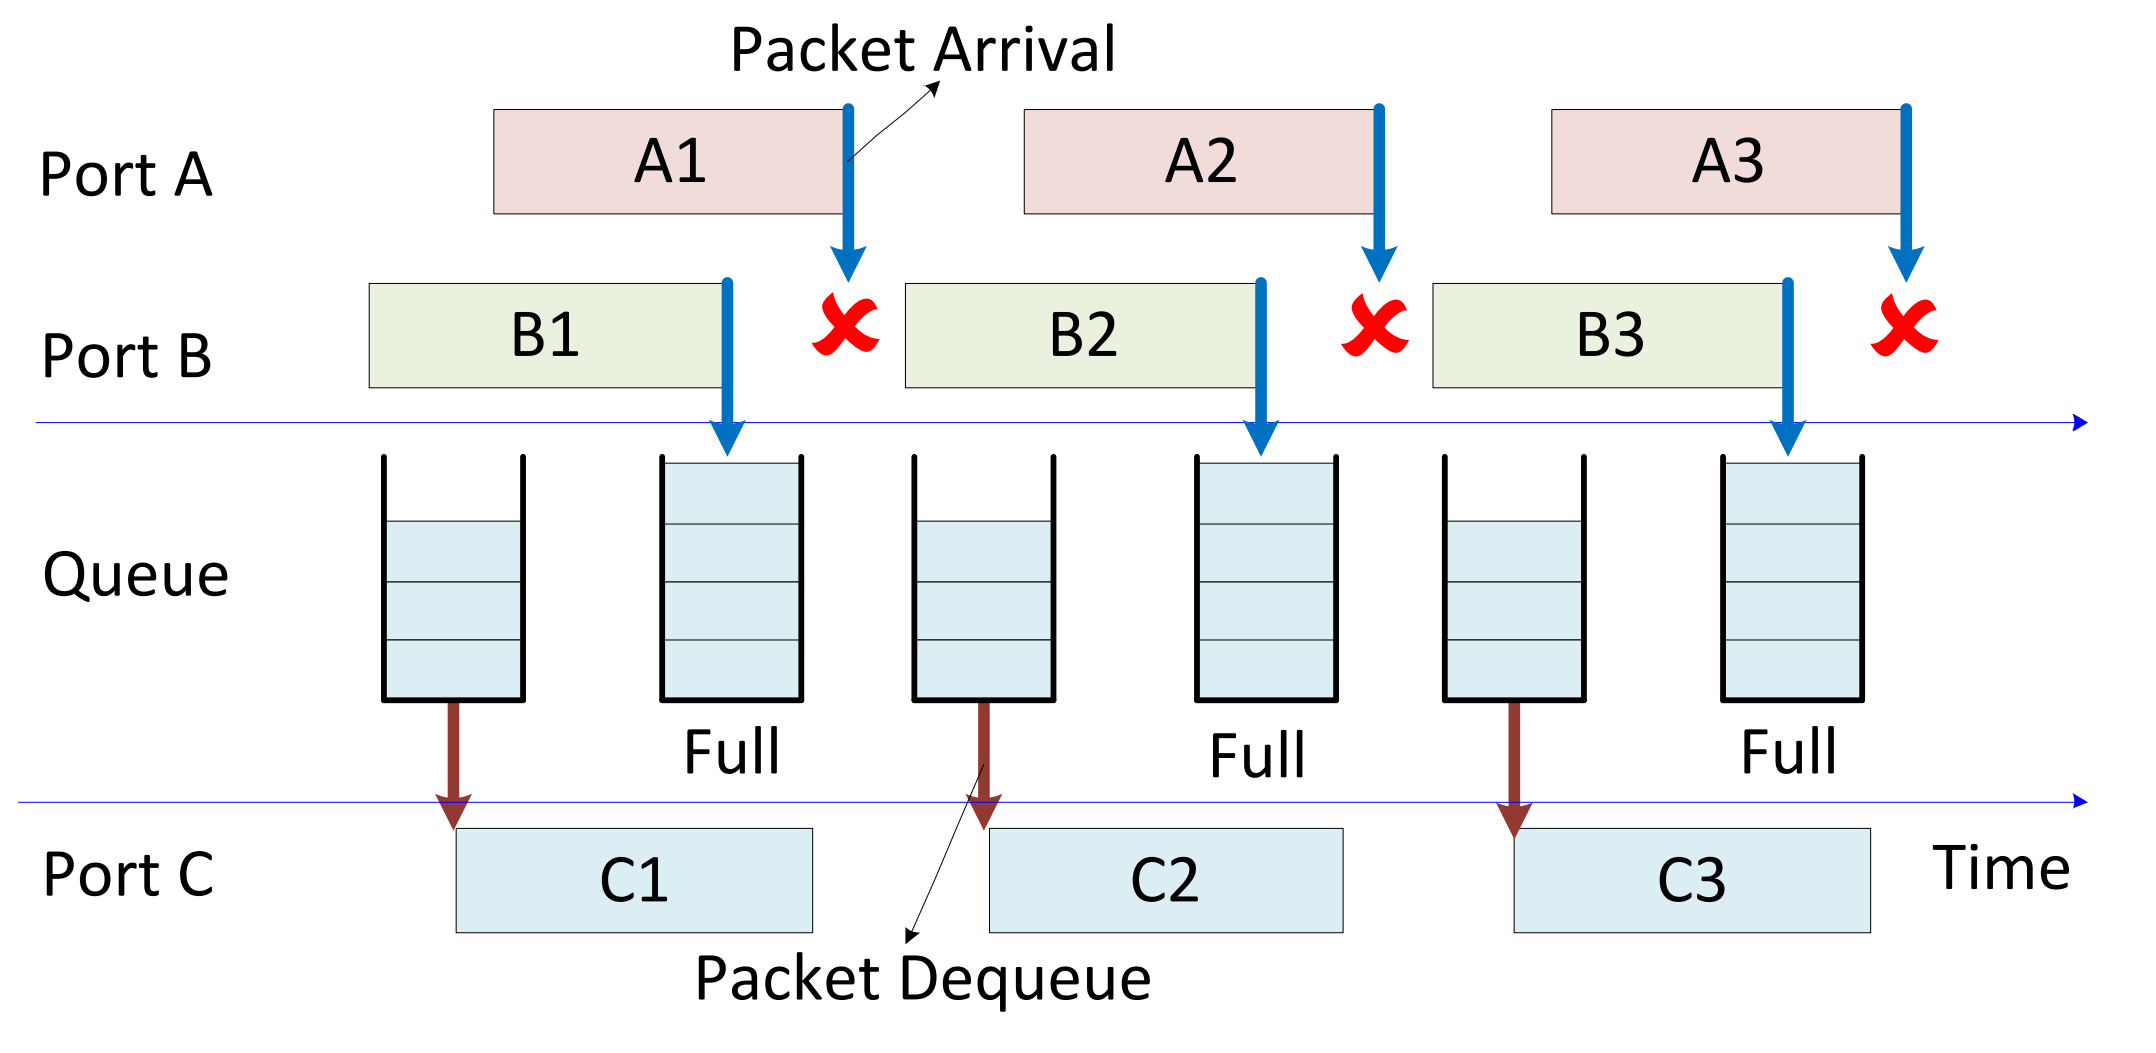
\includegraphics[width=1\textwidth]{figures/TCP_Outcast_Example.png}
    \caption{Reproducción conceptual de Port Blackout tomada de \cite{Prakash_Outcast_2012}. El puerto C es el de salida hacia el \textit{receiver}, mientras que los puertos A y B son de entrada. Vemos cómo la cola se llena con los paquetes provenientes de B, mientras que se rechaza a los provenientes de A.}
    \label{fig:port_blackout_example}
\end{figure}

Cuando un puerto de un \textit{switch} está afectado por Port Blackout, las conexiones que pasan a través de él en la dirección del \textit{blackout} observan ráfagas de paquetes descartados.

Los paquetes descartados por el \textit{blackout} pueden tener un efecto catastrófico, dependiendo de la cantidad de conexiones entrantes en el puerto que lo sufre. Si hay una única conexión, la misma percibirá una ráfaga de \textit{timeouts} que generaran la caida de la ventana de congestión y, por ende, del \textit{throughput}. En un caso con múltiples conexiones entrantes, la pérdida de paquetes se distribuye entre ellas, generando un efecto más leve.

En resumen, TCP Outcast es un problema que nace con la generación de Port Blackout en la capa de enlace, asimismo generado por un conjunto de condiciones causadas por la capa de aplicación y es, al igual que Incast, empeorado por los mecanismos de control de congestión de TCP, en la capa de transporte.

\section{Soluciones} \label{solutions}

% TODO: https://ieeexplore.ieee.org/document/8485935

El objetivo de esta sección es exponer algunas de las muchas soluciones que se han dado en la literatura para TCP Incast. El tema tiene una literatura amplia y variada: desde cambios simples como modificar parámetros del sistema operativo, a nuevas versiones de TCP con cambios que afectan más allá de la capa de transporte.

La filosofía para la selección de los protocolos expuestos apunta a mostrar una selección amplia de ideas, más que a la búsqueda de la mejor solución. Esto es consecuencia directa de leer los artículos: dejan muy claro que no hay una solución óptima, sino más bien múltiples conjuntos de \textit{trade-offs}, del cual debemos elegir uno.

\subsection{Capa de Aplicación}

La forma, quizás más fácil, de evitar un mal comportamiento de TCP es en principio evitando el patrón que lo genera en primer lugar. En efecto, hubo intentos de "mitigar" TCP Incast simplemente no generándolo, y esta es la aproximación al problema que toman las soluciones en capa de aplicación.

Este tipo de soluciones tienen la gran ventaja de poder ser a medida: cada aplicación puede ver de qué forma evitar Incast según tenga sentido en su dominio. En efecto, esta salida ha sido la que parecen haber tomado sistemas como Panasas, y tienen a favor el hecho de tener testimonios de éxito.

Por otro lado, una solución a este nivel es de poca generalidad, y además cualquier mecanismo en capa de aplicación tiene la desventaja de no poder operar con información de bajo nivel de TCP, por lo que a priori parecería ser más difícil lograr maximizar el \textit{throughput}, dado que no hay información sobre la red.

\subsubsection{Aumento de \textit{Server Request Unit}}

\citet{Phanishayee_Throughput_2008} experimentan con la idea de aumentar el tamaño del SRU. De esta forma, la cantidad de tiempo en el que el enlace está desocupado se vuelve mucho menor, ya que los tiempos muertos de espera por \textit{timeout} se ven tomados transfiriendo más datos del SRU.

Esta técnica funciona muy bien si sólo miramos \textit{throughput}, inclusive cuando el número de servidores llega a los varios cientos \cite{Ke_SchedulingDataRequests_2012}. Además, en sistemas de \textit{storage} distribuidos basados en discos rígidos tradicionales, un mayor SRU implica mayor eficiencia en las operaciones de lectura, ya que la lectura se realizará de forma contigua. 

Sin embargo -y este es un problema que afecta sin importar el tipo de disco rígido-, un mayor SRU también implica \textit{locks} tomados sobre mayores cantidades de datos, lo que podría generar congestión en escrituras contiguas en paralelo. Fuera de eso, las aplicaciones tienden a utilizar un SRU pequeño por problemas de presión de memoria: cuando se solicita un mayor tamaño, el cliente debe reservar memoria para poder recibir todos los datos, y esto suele llevar a fallos a nivel \textit{kernel} \cite{Kulkarni_Probabilistic_2011}.

\subsubsection{Aumento de \textit{Block Size}}

\citet{Krevat_ApplicationLevelApproaches_2007} proponen solicitar una mayor cantidad de información, pero a un menor subconjunto de servidores, es decir, limitando el paralelismo. Al haber una menor cantidad de \textit{workers} enviando datos en simultáneo, si bien seguimos siendo susceptibles a Incast, es más improbable que suceda.

Más aun, es posible investigar qué cantidad de servidores comunicándose concurrentemente generan la caída de \textit{goodput} y evitarla. De hecho, los autores reportan que Panasas \cite{Nagle_Panasas_2004} utiliza una estrategia basada en efectivamente restringir la cantidad de servidores que responden en simultaneo.

Cabe destacar que esta forma de resolver el problema puede no ser viable para sistemas donde lo que se está distribuyendo es cómputo, en lugar de lectura de datos. En el caso de cómputo, utilizar una menor cantidad de servidores implica, en un paradigma como MapReduce, menor grado de paralelismo y, por ende, mayor cantidad de tiempo para resolver la misma cantidad de trabajo. Es decir, tenemos un \textit{trade-off}.

En efecto, todas las plataformas populares de cómputo distribuido proveen una forma de limitar el paralelismo de manera trivial, con un parámetro en el estilo de "máxima cantidad de \textit{workers} trabajando en paralelo".

Si bien esta forma es barata de implementar y utilizar, queda claro que en la práctica es difícil: a priori no podemos saber cuántas conexiones en simultáneo pueden pasar por el cuello de botella en un momento determinado, por lo que es difícil elegir el parámetro de forma que evite Incast.

Por supuesto, hay formas de estimar la cantidad de servidores en simultaneo \cite{Zheng_BlockSizeExp_2011} \cite{Chen_BlockSizeExpV2_2012} basadas en modelos de \textit{throughput} en función de las variables relevantes al problema, como \textit{block size} y SRU. Sin embargo, estos modelos son muy limitados, y no toman en consideración el estado actual de la red, por lo que no tienen información sobre la congestión que ya podría estar sucediendo. Además, en toda la literatura observada estos modelos son creados para una versión específica de TCP, y comprobados únicamente a través de simulaciones, por lo que podría argumentarse una falta de generalidad, así como de experiencia práctica con ellos.

\subsubsection{Application-Level Scheduling}

Como se mencionó anteriormente, el principal causante de TCP Incast son los \textit{timeouts}. Podlesny et. al \cite{Podlesny_ApplicationLevelScheduling_2012} sugieren una solución donde el \textit{scheduler} del sistema distribuido organiza los servidores de forma tal que no ocasionen pérdida de paquetes, por ende evitando la generación de \textit{timeouts}.

Para esto, la idea clave es que se puede utilizar la dinámica de Slow Start de TCP para obtener una cota superior a la máxima cantidad de flujos en paralelo que pueden ser soportados sin pérdida de paquetes. Es decir, podemos encontrar una cota para el paralelismo de forma dinámica.

Esta información es utilizada por el \textit{scheduler}, uno por \textit{rack} el \textit{data center}, para dividir a los servidores en grupos que coordinan su respuesta en ráfagas, cada grupo enviando todos en simultaneo. Como la cantidad de servidores en el grupo está calculada para que la ráfaga no genere pérdida de paquetes, en ningún momento se generan \textit{timeouts}. Esta solución ha obtenido buenos resultados en simulaciones; sin embargo, cabe destacar que:

\begin{itemize}
    \item Requiere coordinación entre todos los servidores en un \textit{rack}, que es caro.
    
    \item Utiliza información a nivel de transporte (es decir, de TCP) para tomar una decisión a nivel aplicación. Este tipo de información no es tradicionalmente accesible por fuera del \textit{kernel} sin utilizar módulos adicionales. 
    
    \item La cantidad de servidores por grupo está elegida con cuidado para no sobrepasar la capacidad de la red. Como las tareas de MapReduce son tradicionalmente de larga duración, también quiere decir que ese estimativo de la capacidad de la red puede quedar desactualizado, y por ende estar subestimando.
    
    \item Dado que la solución no fue puesta en producción en una red no simulada, queda en duda la utilidad práctica.
\end{itemize}

\subsubsection{Global Scheduling}

En el mismo espíritu que las otras metodologías de la capa de aplicación, la idea detrás de Global Scheduling es limitar la cantidad de servidores que pueden establecer conexiones en simultaneo. La diferencia clave con respecto a las otras iniciativas es que, en este caso, se utiliza una primitiva denominada \textit{SRU token}, muy similar a un semáforo.

Un \textit{SRU Token} es metafóricamente un permiso para enviar datos a un cliente dado. Cuando un servidor desea enviar datos a otro, debe obtener un \textit{token} del \textit{receiver} para poder iniciar la transferencia. Por supuesto, la cantidad de \textit{tokens} disponibles para cada receptor está limitada para que no pueda generarse Incast. No es factible elegir la cantidad de \textit{tokens} para un cliente manualmente, por ende se precisa de algún modelo para determinar este número; la literatura no se explaya sobre qué modelo podría utilizarse.

Esta idea aparece brevemente mencionada en \cite{Krevat_ApplicationLevelApproaches_2007}, así como en varios otros artículos, pero no hay reportes ni de simulaciones, ni de puestas en producción de aplicaciones con este tipo de solución a fines de evitar Incast.

\subsection{Capa de Transporte}

Hay múltiples formas de categorizar a las soluciones para TCP Incast a nivel de capa de transporte. Tal vez la más general es mirando qué intentan resolver: hay algunas que buscan evitar el problema, y otras cuyo foco es mitigarlo una vez que ya está sucediendo.

En las que buscan evitarlo, el foco está puesto en evitar la generación de \textit{timeouts}, ya que fueron identificados como los mayores responsables de TCP Incast. En las que buscan mitigarlo, la clave está en reducir la penalidad de los \textit{timeouts} una vez que ya están sucediendo. La mayoría de las soluciones van por la primer vertiente.

Otra forma de categorizar a las soluciones es la metodología de resolución; en este caso tenemos, ordenadas por complejidad ascendente:

\begin{enumerate}
    \item Cambio de parámetros en TCP, donde la idea clave es ajustar de alguna manera los parámetros estándar de las implementaciones para que reflejen mejor la situación en un \textit{data center}.
    
    \item Modificaciones en los algoritmos de control de congestión de TCP para tomar en consideración la posibilidad de Incast.
    
    \item Cambios más grandes a nivel de protocolo, donde se llega a agregar información de congestión a los paquetes en los puntos intermedios de la conexión, o a requerir cambios significativos de la implementación.
\end{enumerate}

% Queda claro que, en el primer caso, el costo es relativamente bajo siendo reducido a un cambio de configuración. En el segundo caso los requisitos son sustancialmente mayores, ya que necesitamos un soporte a nivel \textit{kernel} de estos protocolos, lo que requiere un \textit{deploy} en todo el \textit{data center}. El tercer y último caso es aun peor: además de requerir cambios en cada servidor, es posible que haya cambios en los \textit{switches} intermedios.

\subsubsection{Cambio de Parámetros}

Este tipo de soluciones evitan hacer cambios grandes, a través de sólo ajustar los parámetros expuestos por la implementación para atacar Incast.

Cabe destacar que un patrón común entre estas soluciones es el hecho de que tienen que ver con intentar disminuir el costo de los \textit{timeouts}. Es decir, de bajar las penalidades de TCP por haber incurrido un \textit{timeout}, o de lograr una recuperación más rápido.

La gran ventaja con este tipo de soluciones es que son muy baratas de implementar, y tienen el beneficio de no requerir cambios en otras capas.

Sin embargo, ninguna de estas soluciones logra eliminar el problema, solamente permiten soportar una mayor cantidad de servidores en paralelo antes de que se reproduzca. Además, en ninguno de los casos hay reportes de que hayan sido utilizadas en \textit{data centers} reales, y por ende hay una falta de evidencia de que estas soluciones funcionen bien interactuando con \textit{hosts} fuera del \textit{data center}, o información sobre cómo interactúan en un ambiente productivo.

\paragraph{Menor RTO Timer}

Recordemos que hay dos mecanismos principales a través de los cuales TCP decide retransmitir un paquete, o un conjunto de ellos:

En primer lugar, por el \textit{RTO timer}: TCP mantiene, para cada conexión, un estimador del RTT que es utilizado para computar el tiempo que puede permanecer un paquete hasta considerarse en estado de \textit{timeout}. Si un paquete no recibe un ACK antes de que el \textit{timer} expire, entonces el paquete será reenviado. Las implementaciones tienen un valor mínimo para este \textit{timer}, denominado $\text{RTO}_{\text{min}}$.

En segundo lugar, a través del mecanismo de Fast Retransmit, por el cual 3 ACKs duplicados son tomados como una señal de que se debe volver a enviar el paquete referido por el ACK.

En un \textit{data center network}, el RTT es mucho más bajo que en la Internet: en el orden de decenas a cientos de microsegundos, contra decenas a cientos de milisegundos dependiendo de dónde a dónde es la conexión. Por ende, el valor por defecto de $\text{RTO}_{\text{min}}$ (en Linux, 200ms), pensado para el entorno de Internet, deja de ser razonable en un ambiente de \textit{data center}. En la práctica, un mal valor de $\text{RTO}_{\text{min}}$ puede generar:

\begin{itemize}
    \item Si es demasiado bajo, \textit{timeouts} espurios y paquetes retransmitidos sin sentido. Además, cuando el \textit{timer} expira, TCP entra en Slow Start, llevando a subestimar la capacidad de la conexión \cite{Sargent_Computing_2011}.
    
    \item Si es demasiado alto, se demora demasiado en retransmitir paquetes que en efecto fueron perdidos, lo que penaliza el \textit{throughput}, ya que la ventana deslizante de TCP no podrá moverse. 
\end{itemize}

Se realizaron una gran cantidad de experimentos con la idea de disminuir $\text{RTO}_{\text{min}}$, y se ha verificado que reducirlo -inclusive hasta un orden de magnitud- lleva a una mejora en el \textit{goodput} a nivel aplicación \cite{Phanishayee_Throughput_2008} \cite{Chen_Understanding_2009} \cite{Vasudevan_FineGradinedRetrans_2009} \cite{Ke_SchedulingDataRequests_2012} \cite{Chen_Comprehensive_2015} \cite{Osada_RTO_2017}.

Esta solución es difícil de implementar: al día de hoy, los \textit{timers} de las implementaciones populares de TCP pueden mantenerse precisos en el orden de los milisegundos; todos los autores reportan que es necesario o bien soporte de hardware (que no existe), o bien relojes simulados por software, que son ineficientes de implementar con esos requisitos de granularidad.

Cabe destacar que, a priori, esta solución tiene el problema de complicar la comunicación fuera del \textit{data center}: si bien el valor de $\text{RTO}_{\text{min}}$ puede ser adecuado dentro de un \textit{rack}, cualquier conexión fuera del \textit{data center} sufrirá los problemas de tener un valor demasiado bajo.

\citet{Vasudevan_FineGradinedRetrans_2009} realizaron una investigación más profunda al respecto, implementando soporte para \textit{timers} de alta resolución en Linux con soporte de hardware, y realizando pruebas en un \textit{cluster} con hasta 47 servidores respondiendo en simultaneo. En efecto, no sólo replicaron los resultados, sino que además hicieron un intento de eliminar el $\text{RTO}_{\text{min}}$, con el resultado muy satisfactorio de no ver Incast con el máximo de servidores.

Es decir, los experimentos realizados muestran que Incast sigue sucediendo a pesar de haber decrementado el valor: logra soportar una mayor cantidad de servidores en simultaneo y mantener un mayor \textit{goodput} luego de que haya sucedido, pero no lo evita, excepto en el caso del borrado del $\text{RTO}_{\text{min}}$. Además, realizaron un conjunto de experimentos a fin de demostrar que su solución no genera conflictos en WAN. Estos dieron un resultado positivo, mas están lejos de ser exhaustivos.

\paragraph{Desactivar Delayed ACK}

Esta es una conocida técnica utilizada por algunas implementaciones de TCP (viene por defecto activado en la mayoría de las distribuciones de Linux) a través de la cual un \textit{host} que recibe datos en una conexión TCP puede agrupar ACKs para múltiples paquetes en un único ACK, efectivamente evitando tener que enviar un ACK por paquete y por ende disminuyendo el costo del protocolo.

La idea es que el receptor de un paquete puede esperar hasta 200 ms (en Linux, 40 ms) para enviar el ACK correspondiente; además, debe enviar un ACK cada dos paquetes de tamaño MSS (\textit{Maximum Segment Size}). Esto permite decrementar ampliamente la cantidad de paquetes que envía el lado receptor.

También se ha realizado experimentación sobre la idea de desactivarlo, con argumentos de que puede producir patrones de comunicación que empeoran el \textit{goodput} en una situación de Incast \cite{Phanishayee_Throughput_2008} \cite{Vasudevan_FineGradinedRetrans_2009}.

Cuando $\text{RTO}_{\text{min}}$ está presente, no se observaron cambios significativos en el \textit{goodput}; pero cuando el mismo fue eliminado, se comenzó a ver mejoras: con un valor cada vez más chico para el \textit{timer}, hasta eliminarlo.

\paragraph{Eliminar Exponential Backoff}

\citet{Zheng_ExpBackoff_2011} encontraron que el Exponential Backoff utilizado para computar el tiempo de \textit{timeout} para un paquete que fue descartado sucesivas veces era invocado cada vez más a medida que se agregaban servidores. 

Es decir, que los \textit{timeouts} de Incast se repiten múltiples veces cuando agregamos más servidores, generando mayor \textit{backoff} en cada vez, y de esta manera poniendo el freno a la ventana deslizante de TCP. Fuera de eso, encontraron que reducir $\text{RTO}_{\text{min}}$ genera que la se produzca menos \textit{backoff} con una menor cantidad de servidores, pero que el efecto se vuelve aun peor cuando se genera Incast.

Experimentaron entonces con eliminar Exponential Backoff; los resultados fueron altamente positivos: con un $\text{RTO}_{\text{min}}$ de 1 ms, no se reprodujo Incast hasta los 512 servidores en simultaneo. El argumento que presentan los autores es que esta técnica reduce el \textit{burstiness} de TCP en este entorno, logrando una reducción del \textit{waiting time} del cliente antes de poder solicitar el próximo bloque de datos.

Cabe destacar que no se realizaron experimentos sobre cómo esto interactúa en una WAN, donde sí podría ser necesario el uso de la técnica.

\paragraph{Menor MTU}

\citet{Zhang_MTU_2011} proponen reducir el Maximum Transmission Unit (MTU) de la interfaz de red. De esta forma, se producen paquetes más pequeños, generando que el \textit{buffer} del \textit{switch} pueda mantener más paquetes, y por ende reduciendo el número de ellos que son descartados, que es equivalente a decir que hay una menor cantidad de \textit{timeouts}.

Si bien este método no logra eliminar Incast, sí logra aumentar la cantidad de servidores en paralelo que son necesarios para caer en Incast.

Hay técnicas más recientes \cite{Huang_MTUVarV1_2015} \cite{Huang_MTUVar_2018} de ideas similares: pasan a utilizar un tamaño de paquete variable, donde el mismo está determinado por un modelo cuyo propósito es maximizar el \textit{goodput} y minimizar la probabilidad de Incast. Los resultados son mejoras de hasta 26x en el \textit{goodput} de algunas variantes de TCP pensadas para el \textit{data center}.

\subsubsection{Algoritmia para Control de Congestión}

% TODO: https://ieeexplore.ieee.org/document/7543904

\paragraph{Retransmisión Probabilística}

\citet{Kulkarni_Probabilistic_2011} proponen una técnica cuya idea clave es que podemos utilizar paquetes marcados para obtener información sobre el estado del \textit{switch} congestionado. El algoritmo modifica tanto el receptor como el emisor:

\begin{itemize}
    \item El \textit{sender} corre un \textit{thread} que marca con un probabilidad $p$ al paquete más nuevo sin ACK recibido y lo retransmite.
    
    \item El \textit{receiver}, al recibir un paquete, primero se fija si recibe un paquete duplicado; si no lo está, entonces continua con su flujo normal, en el caso contrario, chequea si está marcado o no. En el caso en que sí, envía \textit{duplicate ACKs} para que el \textit{sender} entre en Fast Retransmit.
    
    \item El sender, previo a entrar en Fast Retransmit, desactiva el \textit{thread} de marcado de paquetes.
\end{itemize}

Imaginemos un \textit{switch} que recibe un paquete marcado; el mismo puede estar en tres estados: previo a un episodio de congestión, sufriendo congestión, o habiendo pasado un estado de congestión. En el primer caso, el paquete retransmitido va a ser descartado por ser duplicado, respondiendo con un ACK; en el segundo caso, el paquete retransmitido se descarta en el \textit{switch}; en el tercer caso, el paquete retransmitido sería la primer copia que vería el receptor, generando Fast Retransmit del lado del emisor.

Entonces, con esta metodología en cuanto el \textit{switch} tenga espacio disponible en su \textit{buffer}, el emisor enviará todos los paquetes faltantes, de esta forma destrabando la ventana de congestión y saliendo de la situación de congestión.

Los autores reportan resultados positivos, donde encuentran que pequeños valores de $p$ logran eliminar Incast. Sin embargo, todos los resultados provienen de simulaciones, sin información sobre cómo se comportaría tal solución en un entorno productivo.

\paragraph{Session-Aware Congestion Control}

\citet{Li_SACC_2016} proponen que el receptor mida la cantidad y velocidad de datos que le están siendo transmitidos por cada emisor, y forzar \textit{fairness} enviando un paquete marcado a los emisores que estén acaparando el enlace para que reduzcan su ventana de congestión.

De esta forma, permite que las conexiones que están objetivamente más lejos de terminar enviando datos logren alcanzar a las otras, reduciendo el efecto en el tiempo de transmisión total (recordemos que los en Incast, los bloques están sincronizados en barrera).

El algoritmo logra mejorar los resultados aplicado a TCP y a DCTCP: los autores muestran mejoras claras de \textit{goodput}, y una reducción de algunos milisegundos en el tiempo requerido para completar la transmisión. Sin embargo, el algoritmo requiere soporte por parte de los \textit{switches} intermedios, y todos los resultados expuestos son únicamente resultados de simulaciones.

\subsubsection{Protocolos Específicos}

Esta clase de soluciones se caracterizan por ser cambios grandes, donde se cambia significativamente el funcionamiento de TCP, e inclusive se imponen requisitos en otras capas. La idea en estos casos es siempre atacar desde raíz el problema. Al ser soluciones más integrales para el problema, también logran resultados más fuertes, pero con un mayor costo implementativo.

Por supuesto, hay una gran cantidad de variaciones de TCP, todas con ligeros ajustes para evitar distintos comportamientos patológicos. En este trabajo nos limitamos a relatar algunas de las que son frecuentemente citadas por la literatura sobre Incast, con un foco en mostrar variedad de ideas. 

\paragraph{DCTCP}

\citet{Alizadeh_DCTCP_2010} proponen Data Center TCP, un protocolo basado en Explicit Congestion Notification (ECN) a nivel de \textit{switches} de Ethernet para proveer información a las dos puntas de una conexión TCP. Con conocimiento del estado de congestión en los \textit{switches} intermedios, DCTCP estima un factor de congestión, que luego utiliza para reducir la ventana deslizante desde el lado emisor. De esta forma, logran evitar que suceda la congestión en primer lugar -por ende evitando los \textit{timeouts} que generan Incast de raíz-, y recuperarse de ella rápidamente cuando es inevitable.

En la versión vainilla de TCP, el emisor reacciona a un evento que notifica congestión -usualmente \textit{timeouts}- reduciendo la ventana de congestión a la mitad; la idea clave de este protocolo es que se puede utilizar ECN para obtener un estimador de "cuánta congestión está sucediendo", y de esta forma reducir la ventana a un punto operativo más preciso.

Con esta intención, los \textit{switches} utilizan una variante de Random Early Detection (RED) \cite{Floyd_RED_1993}, donde marcan los paquetes que pasan a través de ellos con un bit de Congestion Experienced (CE) en cuanto sus \textit{buffers} están ocupados más de un cierto valor (es decir, los límites inferiores y superiores son equivalentes, la probabilidad de marcado es 1, y el mismo es basado en el valor instantáneo en lugar del promedio).

Luego, se aplica una modificación en el lado receptor, donde básicamente se adapta \textit{Delayed ACK} para poder enviarle al emisor la cantidad de paquetes que fueron marcados, codificados como una secuencia de ACKs.

Finalmente, se adapta al emisor para poder decodificar la secuencia de ACKs en un estimador del factor de congestión actual en la red, y se utiliza este estimador para reducir la ventana de congestión. Cuando el factor de congestión $\alpha$ es alto (cerca de 1), la reducción es equivalente a la de TCP, es decir, una división por 2, y cuando $\alpha$ es bajo (cerca de 0), prácticamente no habrá reducción.

Los autores realizaron una gran cantidad de experimentos sobre un \textit{data center} productivo, con aplicaciones reales, y encontraron resultados muy positivos: una disminución drástica de la cantidad de paquetes encolados, mejoras sustanciales en la latencia de las respuestas y, por supuesto, la eliminación de Incast.

Cabe destacar, sin embargo, que no hacen referencia sobre cómo impacta DCTCP en las conexiones hacia clientes fuera del \textit{data center}, y que el uso productivo del protocolo requiere \textit{switches} con ECN.

\paragraph{ICTCP}

\citet{Wu_ICTCP_2010} desarrollaron Incast Congestion Control for TCP (ICTCP), es una modificación de TCP en el receptor por la cual el mismo pasa a manejar su ventana de congestión para evitar Incast. La idea básica del algoritmo es mantener un estimativo de cuál es el ancho de banda disponible en la interfaz, y luego adaptar las ventanas del receptor en todas las conexiones para que se logre llenar el ancho de banda, pero con incrementos conservadores para no generar \textit{timeouts} que puedan llevar a Incast.

Hay tres observaciones clave que motivan los cambios en el algoritmo y funcionan como principios de diseño:

\begin{enumerate}
    \item El receptor puede utilizar el ancho de banda disponible como señal para activar el control de congestión. Además, al realizar incrementos en las ventanas de congestión puede predecir si hay suficiente ancho de banda para soportar el tráfico; más aun, puede hacer esto inclusive si el incremento es en múltiples conexiones.
    
    \item Si consideramos un esquema que administra las conexiones de forma global, debemos tener en cuenta el RTT de cada conexión al momento de realizar ajustes; ya que cada conexión puede tener un distinto valor, y por ende los cambios de ventana y sus resultados se verán en tiempos diferentes.
    
    \item Es posible ajustar la ventana dependiendo de el estado de congestión del enlace y los requisitos de aplicación. Entonces, deberíamos no restringir el \textit{throughput} cuando hay ancho de banda disponible, y regularlo cuando sucede Incast.
\end{enumerate}

Observemos que para poder llevar a cabo el primer principio necesitamos información global a la interfaz, respectivamente el ancho de banda disponible. Para obtener este dato, los autores dividen el tiempo en bloques de longitud $T$, estimando el ancho de banda disponible en un bloque, y usando el dato en el próximo bloque para actualizar las ventanas. Es decir, se actualizan las ventanas cada 2 bloques de tiempo.

Cabe destacar que el receptor tiene la posibilidad de controlar el envío de datos del emisor únicamente cuando debe enviar un paquete, usualmente ACK. Como ICTCP no genera tráfico adicional, esto quiere decir que recién en 2*RTT se verán aplicados los cambios de ventana: precisamos un RTT para que el emisor se entere del cambio de ventana, y un RTT adicional para ver el cambio de \textit{throughput}. Además, como el cambio de ventana sólo puede suceder durante un "segundo bloque", es posible que una conexión individual pierda la oportunidad de adaptar su ventana. Este esquema de división del tiempo nos permite llevar a cabo el segundo principio de diseño.

Al momento de controlar la ventana de una conexión particular, los autores toman la idea de TCP Vegas, pero aplicada a un coeficiente distinto y sobre el receptor: se estiman el \textit{throughput} actual y el esperado, y se mira qué tan cerca está el actual del esperado:

\begin{itemize}
    \item Si está muy abajo, se incrementa la ventana, asumiendo que estamos en un segundo bloque de tiempo y hay suficiente ancho de banda para soportar el tráfico.
    
    \item Si está muy cerca por 3 o más iteraciones, se achica la ventana 1 MSS, hasta un mínimo de 2*MSS.
    
    \item En otro caso, se mantiene igual.
\end{itemize}

También se adaptan los mecanismos de Slow Start y Congestion Avoidance para tener en cuenta el ancho de banda disponible.

Finalmente, los autores agregan un controlador de \textit{fairness}. Es decir, un mecanismo global que, al detectar que el ancho de banda disponible es demasiado bajo relativo a la capacidad de la red, comienza a achicar las ventanas de las conexiones que son \textit{outliers}.

ICTCP tuvo numerosos casos de experimentación con resultados muy positivos, donde se ve que no sólo evita Incast, prácticamente no suceden \textit{timeouts}, y además logra un muy buen \textit{fairness} entre conexiones al mismo receptor. 

Tiene problemas con el mínimo de la ventana receptora: si es demasiado alta, se corre el riesgo de generar Incast cuando el número de servidores es alto. Los autores postulan la pregunta, pero la responden vagamente.

Otro de los problemas que tiene es la necesidad de mediciones de RTT muy precisas, para lo cual se requiere una implementación de un reloj que es caro en la práctica, al igual que la técnica disminuir el RTO Timer. 

También encuentra problemas en redes de muy alto ancho de banda, ya que si el RTT no decrece proporcionalmente, el incremento de la ventana receptora será muy lento, y demorará en converger. Los autores sugieren aumentar MSS como una posible solución.

\paragraph{GIP}

\citet{Zhang_GIP_2013} crearon Guaranteeing Important Packets (GIP), una modificación de TCP basada en la realización que los \textit{timeouts} en aplicaciones con Incast se generan por pérdidas de paquetes muy específicos, y entonces si podemos asegurar que esos paquetes lleguen siempre bien, no vamos a sufrir Incast.

Para esto, los autores comienzan por identificar los dos tipos de de \textit{timeouts} que generan Incast. Encuentran a la pérdida de una ventana completa como el mayor responsable, y a la falta de ACKs como segundo mayor responsable. 

En el primer caso, observan a partir de sus experimentos que se debe al \textit{burstiness} del tráfico al comienzo de un envío de un SRU. Como todos los servidores comienzan haciendo Slow Start, el \textit{buffer} del \textit{switch} que forma el cuello de botella se llena demasiado rápido, y en algunos casos genera la pérdida de una ventana. En el segundo caso, observan que los paquetes responsables están siempre al final de la transmisión del SRU, ya que no logran llegar antes de que el \textit{retransmission timer} expire; si lo hiciesen, comenzaría Fast Recovery / Fast Retransmit.

A fines de evitar estos problemas, resuelven:

\begin{itemize}
    \item Enviar el último paquete del SRU tres veces. Los autores fundamentan la elección del último paquete en particular con algunos experimentos.
    
    \item Forzar a la conexión a comenzar en Slow Start en cada comienzo de SRU. De esta forma se garantiza que la ventana de congestión de todos los emisores crezca a un valor que no genere Incast.
\end{itemize}

Observemos que estos cambios son únicamente del lado del emisor, y los autores mostraron que relativamente pocos cambios son necesarios para que un sistema operativo POSIX-compliant pueda implementar GIP únicamente para las aplicaciones que lo necesitan. Además, es una solución muy simple al problema.

Los experimentos muestran, además, que es una solución considerablemente mejor a la de reducir el RTO Timer a los valores razonables sin implementar relojes de alta resolución.

Tiene problemas cuando la cantidad de servidores es pequeña (menos de 14), y tiene la desventaja significativa de requerir cambios a nivel aplicación (específicamente notificar al kernel del comienzo y fin de un SRU), que no son típicamente requisitos de protocolos en esta capa. Además, los resultados expuestos son puramente simulados, y no se encontraron reportes con experiencia práctica.

\subsection{Capa de Enlace}

% TODO: https://dl.acm.org/citation.cfm?id=2616451

Hay relativamente poca literatura sobre cómo resolver Incast a través de cambios en la capa de enlace. La gran mayoría se concentra en modificaciones de las capas más arriba, por motivos obvios: esta capa es sustancialmente más cara de cambiar, y por ende menos viable como solución. Como resultado, esta sección tiene considerablemente menos resultados que las anteriores.

\subsubsection{Cambios de Hardware}

Una técnica explorada por múltiples artículos es la de agregar más espacio de \textit{buffer} en los \textit{switches} \cite{Phanishayee_Throughput_2008} \cite{Kulkarni_Probabilistic_2011}. Los resultados son inmediatos, ya que con esto se resuelve el problema de raíz: duplicar el tamaño de \textit{buffer} también duplica la cantidad de servidores que pueden enviar datos en paralelo antes de sufrir Incast, según múltiples simulaciones.

Sin embargo, es importante destacar que esta no es una buena solución: el tamaño de \textit{buffer} es uno de los factores que pueden volver a un \textit{switch} mucho más caro (trae problemas desde consumo de energia, hasta requisitos de memoria y espacio de \textit{buffering} \cite{Shpiner_HCF_2010}); además, reemplazar un \textit{switch} implica un cambio infraestructural, que es de por sí difícil por requerir cambios físicos; y, fundamentalmente, un incremento en el tamaño del \textit{buffer} es acompañado por un aumento del \textit{delay}, que es inaceptable en este tipo de entornos.

\subsubsection{Control de Congestión}

\citet{Zhang_QCN_2011} proponen Fair Quantized Congestion Notification, un esquema de control de congestión a nivel de Ethernet, basado en enviar estimativos de la cantidad de paquetes esperados en el \textit{buffer} del \textit{switch} cuando el mismo es mayor al punto operativo deseado, para que el emisor baje la cantidad de información que está enviando.

Primero explicaremos el protocolo de Quantized Congestion Notification (QCN), que es la base de FQCN, y luego explicaremos los cambios. El protocolo opera en dos lugares: el servidor (o Reaction Point, RP) que envía datos, y los \textit{switches} intermedios (o Congestion Point, CP).

CP tiene como objetivo mantener el \textit{buffer} con una cantidad de datos $Q_{eq}$, y para esto mantiene un estimativo de la severidad de la congestión $F_b$. El mismo se genera muestreando paquetes uniformemente según una probabilidad dependiente de la congestión actual, y calculando:

$$F_b = -(Q_{off} + w * Q_{\delta})$$

Donde $Q_{off} = Q - Q_{eq}, Q_{\delta} = Q - Q_{old}$, $Q$ es el tamaño de la cola en el momento actual, $Q_{old}$ es el tamaño de la cola en la última muestra, y $w = 2$ es un parámetro de la implementación. Intuitivamente, $F_b$ está dando una predicción del exceso en el tamaño de la cola $w$ muestreos a futuro. Si en algún momento $F_b$ es negativo (es decir, estamos por arriba de $Q_{eq}$), se envía un mensaje de control al emisor del paquete muestreado con el valor de $F_b$, cuantizado a 6 bits.

El RP tiene como objetivo mantener el \textit{throughput} más alto posible, sin que los \textit{switches} intermedios se desvíen de su cantidad de datos óptima $Q_{eq}$. Desgranado, el RP tiene tres tareas: ajustar la velocidad de envío de datos cuando llega un mensaje de control, incrementarlo para maximizar el uso del ancho de banda, y sensar el entorno para saber cuando hay ancho de banda adicional disponible.

A este fin, el RP mantiene dos variables claves: TR (o Target Rate), y CR (o Current Rate), que respectivamente dicen cuántos datos debería enviar idealmente, y cuántos datos está enviando actualmente. Luego, tiene múltiples modos operativos que le permiten ajustar estas variables:

\begin{itemize}
    \item Decremento de Velocidad: cuando recibe un mensaje de control, pone $TR = CR$, y $CR = CR (1 - G_d |F_b|)$, donde $G_d$ es una constante para evitar que $CR$ no decrezca más que un 50\%.
    
    \item Incremento de Velocidad: mantiene dos módulos que sirven para este fin:
        \begin{itemize}
            \item Byte Counter (BC): es un contador de la cantidad de bytes transmitidos.
            \item Rate Increase Timer (RIT): es un reloj que es utilizado para elegir cuándo incrementar la velocidad.
        \end{itemize}
    Además, en cualquier momento dado, estos dos módulos pueden estar en alguno de dos estados independientemente: Fast Recover (FR) y Active Increase (AI). Cada módulo está en cierto estado dependiendo de múltiples condiciones. Además, los estados de los módulos determinan el estado del Rate Limiter (RL) que opera para determinar cuál va a ser el incremento:
        \begin{itemize}
            \item Si BC y RIT están en FR, RL está en FR; en cuyo caso cuando se completa un ciclo, se pone $CR = \frac{CR + TR}{2}$, es decir, se acerca el $CR$ al $TR$ poniendose en el punto medio.
            
            \item Si o bien el BC o bien el RIT están en AI, al completarse un ciclo se pone: $TR = TR + R_{AI}, CR = \frac{CR + TR}{2}$, donde $R_{AI}$ es una cantidad de bytes adicional a enviar. Es decir, se incrementa la cantidad de información a enviar.
            
            \item Si BC y RIT están en AI, se entra en Hyper-Active Increase (HAI), donde el incremento de velocidad es mucho mayor, pero con ciertos resguardos para no generar congestión en la red.
        \end{itemize}
\end{itemize}

QCN tiene serios problemas de \textit{fairness} cuando hay múltiples flujos compartiendo un mismo cuello de botella. En Incast, el \textit{goodput} total depende de que todos los flujos logren terminar a tiempo, por la característica de barrera. Por ende, una metodología con estos problemas no es factible como solución.

En FQCN, los autores proponen modificar sólo el algoritmo de CP, agregando información de cada flujo que pasa por el mismo. Entonces, cuando sucede que $F_b < 0$, CP envía el mensaje de control a todos los flujos que están enviando más información de la que deberían, ajustando $F_b$ en cada caso para que el impacto en $CR$ sea mayor cuando hay más \textit{unfairness}. Los experimentos de \cite{Zhang_QCN_2011} muestran que FQCN logra muy buen \textit{throughput} en la situación de Incast.

\subsubsection{Control de Flujo}

% TODO: http://sci-hub.tw/https://ieeexplore.ieee.org/document/7273345

\citet{Phanishayee_Throughput_2008} proponen utilizar Ethernet Flow Control (EFC) para resolver Incast.  La idea clave es que el \textit{switch} que es cuello de botella puede enviar un mensaje de pausa en una interfaz, haciendo que todos los \textit{hosts} en la misma paren de enviar o hacer \textit{forwarding} por una cantidad de tiempo determinada. Durante ese tiempo, el cuello de botella puede reducir la cantidad de paquetes en el \textit{buffer}, así evitando llegar a descartar paquetes. 

Según la simulación que muestran en el artículo, EFC funciona muy bien, pero sólo en la topología estereotípica de Incast, donde son muchos servidores conectados al mismo \textit{switch}, es decir, no funciona en un caso más general.

El problema es lo que llaman \textit{head-of-line blocking}: cuando el \textit{switch} envía un mensaje de pausa, no sólo frena a la conexión que está generando congestión, sino también a todos los otros que estén pasando por el \textit{switch}.

Además, los autores encontraron que las implementaciones de distintas piezas de hardware difieren de formas inconsistentes, lo que vuelve muy difícil mantener este tipo de solución.

Existen ya propuestas que logran resolver el problema, junto con algunos modelos de hardware las implementan, la literatura al respecto excede a este artículo.

\subsubsection{Cambios de Encolamiento}

\citet{Shpiner_HCF_2010} proponen Hashed Credits Fair (HCF), un cambio en la forma de encolar en los paquetes en los \textit{switches} intermedios de forma tal que todas las conexiones logren enviar aproximadamente la misma cantidad de paquetes.

La idea consiste en tener dos colas, una de alta prioridad y una de baja, y utilizar funciones de \textit{hash} para distribuir los paquetes en urnas, cada una con cierta cantidad de créditos disponibles. Cuando el \textit{switch} recibe un paquete, \textit{hashea} el identificador de la conexión y, de haber créditos disponibles y espacio en la cola de alta prioridad, lo encola; en el caso contrario, el paquete es encolado en la de baja prioridad o, si no hay lugar tampoco, descartado. Es decir, cada urna tiene una cantidad de créditos que puede consumir para poner paquetes en la cola de alta prioridad y, por ende, nos permite tener un cierto concepto de \textit{fairness} aproximado. Al momento de transmitir un paquete, el \textit{switch} elige, de ser posible, el primer paquete en la cola de alta prioridad.

Este esquema tiene el beneficio de ser extremadamente simple, de bajo costo, y requerir relativamente pocos cambios en el \textit{switch}. Además, los autores muestran en el artículo que logra mitigar Incast y, dados ligeros cambios, puede además mantener el orden de envío en los paquetes no descartados.

% https://sci-hub.tw/https://ieeexplore.ieee.org/abstract/document/5934923
% \cite{Chen_Understanding_2009} Da un modelo teórico además que ayuda a explicar algunas de las cosas que se ven en Incast
%  https://sci-hub.tw/https://ieeexplore.ieee.org/abstract/document/7218549

% TODO: IDTCP https://dl.acm.org/citation.cfm?id=2598752
% TODO: 2017 https://dl.acm.org/citation.cfm?id=3138199
% TODO: https://dl.acm.org/citation.cfm?id=2330777

% DCTCP Variant: https://dl.acm.org/citation.cfm?id=2884658
% DCTCP Analysis: https://dl.acm.org/citation.cfm?id=2007125

% TCP-CWR: https://dl.acm.org/citation.cfm?id=2950680

% Initiation, Continuation, Termination: https://www.researchgate.net/publication/254463026_Preventing_TCP_incast_throughput_collapse_at_the_initiation_continuation_and_termination

% TODO: Application-Level Sharing https://dl.acm.org/citation.cfm?id=3087559
% TODO: Application-Levle Tokens https://dl.acm.org/citation.cfm?id=2901336

% TODO: Named Data Networking http://sci-hub.tw/https://dl.acm.org/citation.cfm?doid=3226052.3226055
% TODO: + NDN https://dl.acm.org/citation.cfm?id=3226055
\section{Conclusión} \label{conclusion}

% TODO: Survey https://dl.acm.org/citation.cfm?id=2884661
% TODO: Survey https://dl.acm.org/citation.cfm?id=2854809

Los \textit{data centers} se han convertido en una pieza de infraestructura clave para diversas aplicaciones en la nube, y para el guardado de vastas cantidades de datos.

Para lograr que los sean costo efectivos, utilizan las mismas tecnologías que el resto de la Internet, con hardware sacado del estante. Sin embargo, los \textit{data centers} poseen una infraestructura muy distinta a la del resto de la red y, por ende, son susceptibles a problemas únicos del entorno.

TCP Incast es uno de los principales causantes de problemas de \textit{throughput} en estos casos, y de ahí su relevancia como problema de investigación. Es un problema en sí muy rico en su complejidad, y difícil de resolver: al día de hoy continúan produciéndose artículos de investigación al respecto, mostrando claramente que está lejos de ser un problema resuelto.

En este trabajo realizamos un paneo de la literatura sobre TCP Incast en los últimos años; además, resumimos múltiples formas de atacar al problema, desde las capas de Aplicación, Transporte, y Enlace, mostrando una amplia variedad de soluciones con distintas complejidades de implementación y resultados prácticos. En la tabla de la próxima hoja puede verse un resumen de las técnicas exploradas en este trabajo.

\newpage

\newgeometry{left=3cm,bottom=0.5cm, top=0.5cm,right=3cm}

% Please add the following required packages to your document preamble:
% \usepackage{multirow}
% \usepackage{lscape}
\begin{landscape}
\begin{table}[]
\centering
\begin{tabular}{|c|c|l|l|l|}
\hline
\textbf{Capa}                                     & \textbf{Tipo}                                              & \multicolumn{1}{c|}{\textbf{Propuesta}} & \multicolumn{1}{c|}{\textbf{Factibilidad Técnica}}                      & \multicolumn{1}{c|}{\textbf{Costo Implementativo}}                \\ \hline
\multicolumn{1}{|l|}{\multirow{4}{*}{Aplicación}} & \multicolumn{1}{l|}{\multirow{4}{*}{Cambio de Aplicación}} & Aumentar SRU                            & \multirow{2}{*}{Problemas de presión de memoria, fairness. y latencia.} & Bajo. Cambio de un parámetro.                                     \\ \cline{3-3} \cline{5-5} 
\multicolumn{1}{|l|}{}                            & \multicolumn{1}{l|}{}                                      & Aumentar Block Size                     &                                                                         & Bajo. Cambio de un parámetro.                                     \\ \cline{3-5} 
\multicolumn{1}{|l|}{}                            & \multicolumn{1}{l|}{}                                      & Application-Level Scheduling            & Complejo de implementar;                                                & Alto. Requiere planeamiento de la aplicación y cambios de kernel. \\ \cline{3-3} \cline{5-5} 
\multicolumn{1}{|l|}{}                            & \multicolumn{1}{l|}{}                                      & Global Scheduling                       & puede lograr alcanzar el goodput óptimo.                                & Alto. Require planeamiento de la aplicación.                      \\ \hline
\multirow{9}{*}{Transporte}                       & \multirow{4}{*}{Cambio de Parámetros}                      & Menor RTO Timer                         & Logran aminorar el efecto de Incast;                                    & Bajo a Alto. Depende del valor deseado.                           \\ \cline{3-3} \cline{5-5} 
                                                  &                                                            & Desactivar Delayed ACK                  & es claro que no son soluciones ideales.                                 & Bajo. Cambio de un parámetro.                                     \\ \cline{3-3} \cline{5-5} 
                                                  &                                                            & Eliminar Exponential Backoff            & Poca investigación sobre cómo estos                                     & Alto. Requiere actualizar código de fuente.                       \\ \cline{3-3} \cline{5-5} 
                                                  &                                                            & Menor MTU                               & cambios afectan interacciones con Internet.                             & Bajo a Alto. Depende de la técnica.                               \\ \cline{2-5} 
                                                  & \multirow{2}{*}{Control de Congestión}                     & Retransmisión Probabilistica            & Simulaciones con buenos resultados. Sin reportes de uso.                & Alto. Requiere actualizar código de fuente.                       \\ \cline{3-5} 
                                                  &                                                            & Session-Aware Cong. Control             & Simulaciones con buenos resultados. Sin reportes de uso.                & Alto. Requiere actualizar código de fuente.                       \\ \cline{2-5} 
                                                  & \multirow{3}{*}{Protocolos Específicos}                    & DCTCP                                   & Utilizado ampliamente en la práctica.                                   & Intermedio. Requiere deploy en switches.                          \\ \cline{3-5} 
                                                  &                                                            & ICTCP                                   & Simulaciones con buenos resultados. Sin reportes de uso.                & Alto. Requiere actualizar código de fuente.                       \\ \cline{3-5} 
                                                  &                                                            & GIP                                     & Simulaciones con buenos resultados. Sin reportes de uso.                & Alto. Requiere actualizar código de fuente.                       \\ \hline
\multirow{4}{*}{Enlace}                           & Cambio de Hardware                                         & Aumento de Buffer Size                  & Inviable. Costo muy alto.                                               & Muy Alto. Cambio de infraestructura crítica.                      \\ \cline{2-5} 
                                                  & Control de Congestión                                      & Fair Quantized Congestion Notification  & Simulaciones con buenos resultados. Sin reportes de uso.                & Muy Alto. Requiere hardware compatible.                           \\ \cline{2-5} 
                                                  & Control de Flujo                                           & Ethernet Flow Control                   & Buenos resultados en el escenario simple, malos en el real.             & Bajo. Cambio de un parámetro.                                     \\ \cline{2-5} 
                                                  & Cambio de Encolamiento                                     & Hashed Credits Fair                     & Simulaciones con buenos resultados. Sin implementaciones.               & Muy Alto. Cambio de infraestructura crítica.                      \\ \hline
\end{tabular}
\end{table}
\end{landscape}

\restoregeometry

\newpage

\bibliography{readcube_export}{}

\end{document}
